\chapter{Criação do Certificado PGP}

\section{Instalação do GnuPG}
Primeiro, foi necessário instalar o GnuPG no sistema operacional macOS usando o gerenciador de pacotes Homebrew \cite{gnupgdoc}:

\begin{lstlisting}[language=bash]
brew install gnupg
\end{lstlisting}

\section{Geração do Par de Chaves}
Após a instalação, utilizei o comando abaixo para iniciar o processo de geração de chaves \cite{gnupgdoc}:

\begin{lstlisting}[language=bash]
gpg --full-generate-key
\end{lstlisting}

Durante o processo interativo:
\begin{enumerate}
    \item Selecionei o tipo de chave padrão (RSA and RSA)
    \item Defini o tamanho da chave como 3072 bits
    \item Configurei um período de validade de 90 dias
    \item Inseri as seguintes informações pessoais:
    \begin{itemize}
        \item Nome: Joao Cordeiro
        \item E-mail: jschmidtcordeiro@gmail.com
        \item Comentário: Reach out at @cordeiro05 on Instagram or jschmidtcordeiro on GitHub
    \end{itemize}
    \item Criei uma senha forte para proteger a chave privada
\end{enumerate}

\section{Backup da Chave Privada}
Criei um diretório de backup e exportei a chave privada:

\begin{lstlisting}[language=bash]
mkdir -p "4 - Trabalho sobre PGP/backup"
gpg --export-secret-keys --armor 5BD7096F81478AA33F6CB0B4155B13B98FE2E6C8 > "4 - Trabalho sobre PGP/backup/private_key_backup.asc"
\end{lstlisting}

\section{Exportação da Chave Pública}
Exportei a chave pública para um arquivo separado:

\begin{lstlisting}[language=bash]
gpg --export --armor 5BD7096F81478AA33F6CB0B4155B13B98FE2E6C8 > "4 - Trabalho sobre PGP/backup/public_key.asc"
\end{lstlisting}

\section{Publicação no Repositório PGP}
Publiquei a chave pública no servidor de chaves do Ubuntu:

\begin{lstlisting}[language=bash]
gpg --keyserver keyserver.ubuntu.com --send-key 5BD7096F81478AA33F6CB0B4155B13B98FE2E6C8
\end{lstlisting}

\section{Verificação da Publicação}
Para verificar se a chave foi publicada com sucesso, executei:

\begin{lstlisting}[language=bash]
gpg --keyserver keyserver.ubuntu.com --recv-keys 5BD7096F81478AA33F6CB0B4155B13B98FE2E6C8
\end{lstlisting}

A resposta confirmou que a chave está presente no servidor.

\section{Informações da Chave}
\begin{itemize}
    \item \textbf{ID da Chave}: 5BD7096F81478AA33F6CB0B4155B13B98FE2E6C8
    \item \textbf{Tipo}: RSA 3072 bits
    \item \textbf{Data de Criação}: 6 de maio de 2025
    \item \textbf{Data de Expiração}: 4 de agosto de 2025
    \item \textbf{URL para Verificação}: \url{https://keyserver.ubuntu.com/pks/lookup?search=0x5BD7096F81478AA33F6CB0B4155B13B98FE2E6C8&fingerprint=on&op=index}
\end{itemize}

\section{Observações Importantes}
\begin{enumerate}
    \item A chave privada foi armazenada de forma segura
    \item A senha da chave privada foi memorizada
    \item O ID da chave deve ser usado para todas as operações futuras
\end{enumerate}

\section{Experimentos}

\subsection{Criptografia de Mensagem}
Realizei a criptografia de uma imagem para o colega Enzo utilizando sua chave pública:

\begin{lstlisting}[language=bash]
# Importação da chave pública do Enzo
gpg --keyserver keyserver.ubuntu.com --recv-keys 24B83FFEA53408DA

# Criptografia da imagem
gpg --encrypt --recipient 24B83FFEA53408DA cordeiro.jpg --output enzote_criptografado.jpg
\end{lstlisting}

\subsection{Assinatura de Mensagem}
Criei uma assinatura da imagem utilizando minha chave privada:

\begin{lstlisting}[language=bash]
# Assinatura da imagem
gpg --sign cordeiro.jpg
\end{lstlisting}

\subsection{Assinatura Detached}
Gerei uma assinatura separada (detached) da imagem:

\begin{lstlisting}[language=bash]
# Criação da assinatura detached
gpg --detach-sign cordeiro.jpg
\end{lstlisting}

Isso gerou o arquivo \texttt{cordeiro.jpg.sig} contendo apenas a assinatura.

\subsection{Assinatura com Arquivo Original}
Criei uma versão da imagem que inclui tanto o arquivo original quanto a assinatura:

\begin{lstlisting}[language=bash]
# Assinatura com o arquivo original
gpg --sign cordeiro.jpg
\end{lstlisting}

Isso gerou o arquivo \texttt{cordeiro.jpg.gpg} que contém a imagem original e a assinatura.

\section{Resultados dos Experimentos}
\begin{enumerate}
    \item A imagem criptografada (\texttt{enzote\_criptografado.jpg}) só pode ser aberta pelo Enzo usando sua chave privada
    \item A assinatura detached (\texttt{cordeiro.jpg.sig}) permite verificar a autenticidade da imagem original
    \item O arquivo assinado (\texttt{cordeiro.jpg.gpg}) contém tanto a imagem quanto a assinatura em um único arquivo
    \item Todas as operações foram realizadas com sucesso, demonstrando o funcionamento correto do PGP para criptografia e assinatura digital \cite{pgpbest}
\end{enumerate}

\section{Revogação de Certificados}

\section{Criação de um Novo Certificado PGP}
Para realizar o experimento de revogação, criei um novo certificado PGP específico para teste \cite{pgpbest}:

\begin{lstlisting}[language=bash]
gpg --full-generate-key
\end{lstlisting}

\begin{figure}[!htb]
    \centering
    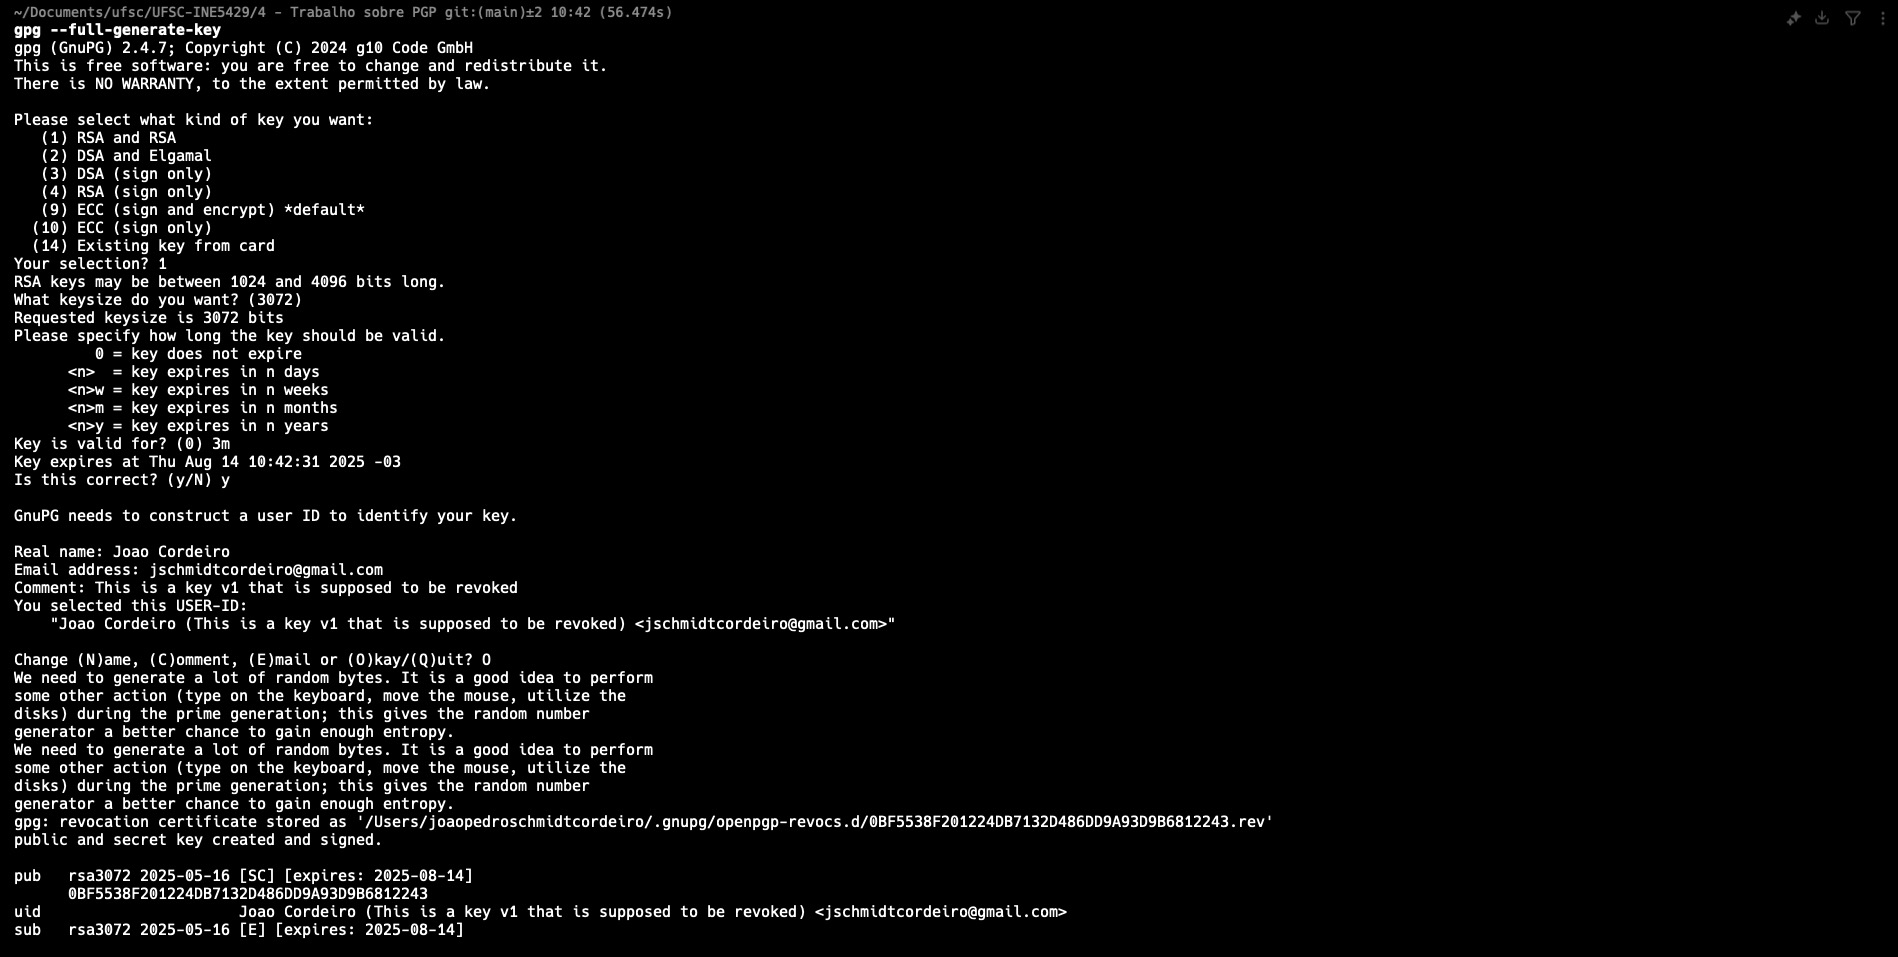
\includegraphics[width=0.8\textwidth]{images/02-criacao_novo_certificado_pgp.jpg}
    \caption{Criação do certificado}
    \label{fig:criacao-cert}
\end{figure}

Durante o processo interativo:
\begin{enumerate}
    \item Selecionei o tipo de chave RSA and RSA (default)
    \item Defini o tamanho da chave como 3072 bits
    \item Configurei um período de validade de 90 dias
    \item Inseri as seguintes informações:
    \begin{itemize}
        \item Nome: Joao Cordeiro
        \item E-mail: jschmidtcordeiro@gmail.com
        \item Comentário: This is a key v1 that is supposed to be revoked
    \end{itemize}
\end{enumerate}

\section{Publicação no Servidor PGP}
Após criar o certificado, publiquei a chave pública no servidor de chaves do Ubuntu:

\begin{lstlisting}[language=bash]
# Obtenho o ID da chave gerada
gpg --list-keys jschmidtcordeiro@gmail.com

# Publico a chave no servidor
gpg --keyserver keyserver.ubuntu.com --send-key 0BF5538F201224DB7132D486DD9A93D9B6812243
\end{lstlisting}

\begin{figure}[!htb]
    \centering
    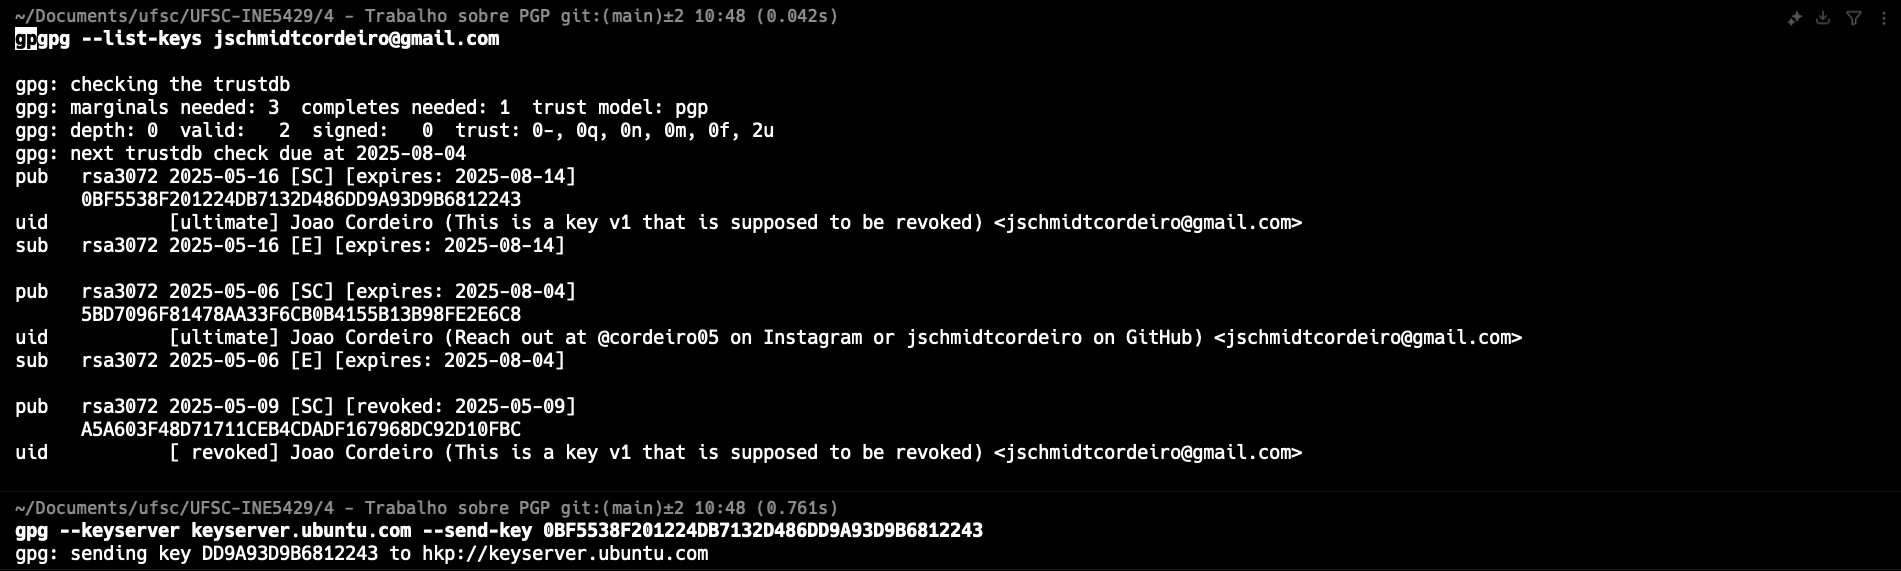
\includegraphics[width=0.8\textwidth]{images/02-publicacao_chave_pgp.jpeg}
    \caption{Publicação da chave}
    \label{fig:publicacao-chave}
\end{figure}

\section{Verificação do Status da Chave}
Para verificar se a chave foi publicada com sucesso:

\begin{lstlisting}[language=bash]
# Atualizo o chaveiro local com informações do servidor
gpg --keyserver keyserver.ubuntu.com --refresh-keys

# Verifico o status da chave específica
gpg --keyserver keyserver.ubuntu.com --recv-keys 0BF5538F201224DB7132D486DD9A93D9B6812243
\end{lstlisting}

\begin{figure}[!htb]
    \centering
    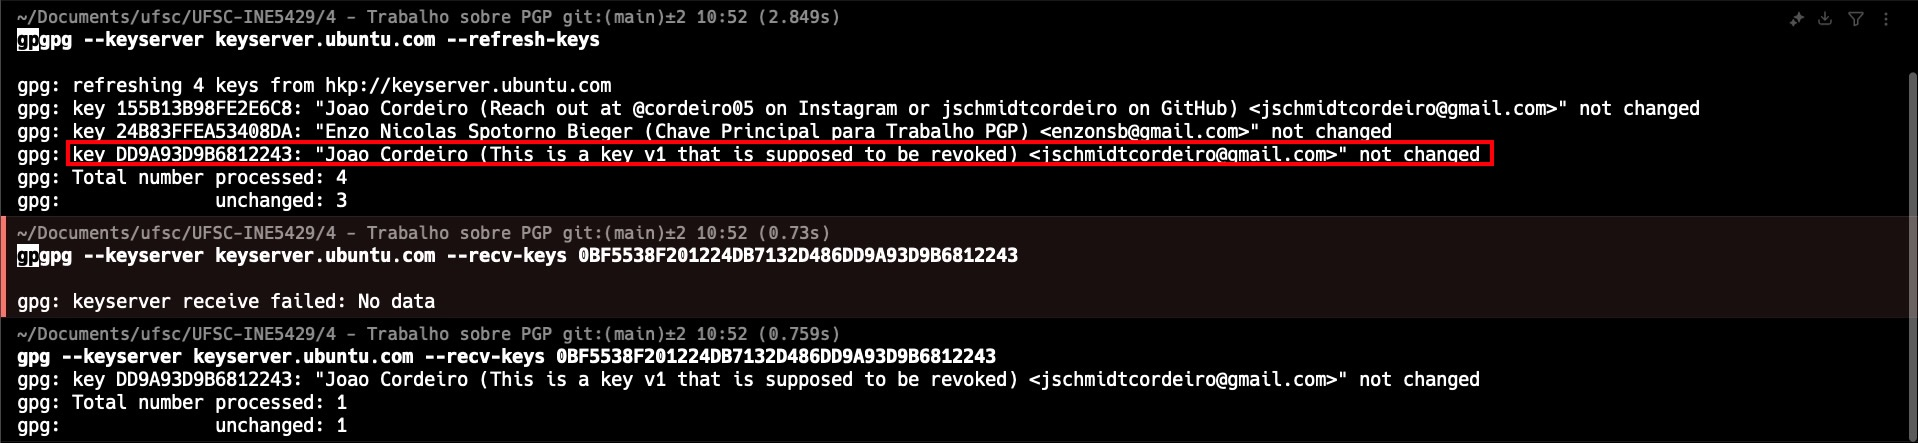
\includegraphics[width=0.8\textwidth]{images/02-verificacao_status_chave.jpeg}
    \caption{Verificação do status da chave}
    \label{fig:verificacao-status}
\end{figure}

\section{Criação do Certificado de Revogação}
Agora, criei um certificado de revogação para a chave \cite{rfc4880}:

\begin{lstlisting}[language=bash]
# Gero o certificado de revogação
gpg --output revocation_cert.asc --gen-revoke 0BF5538F201224DB7132D486DD9A93D9B6812243
\end{lstlisting}

\begin{figure}[!htb]
    \centering
    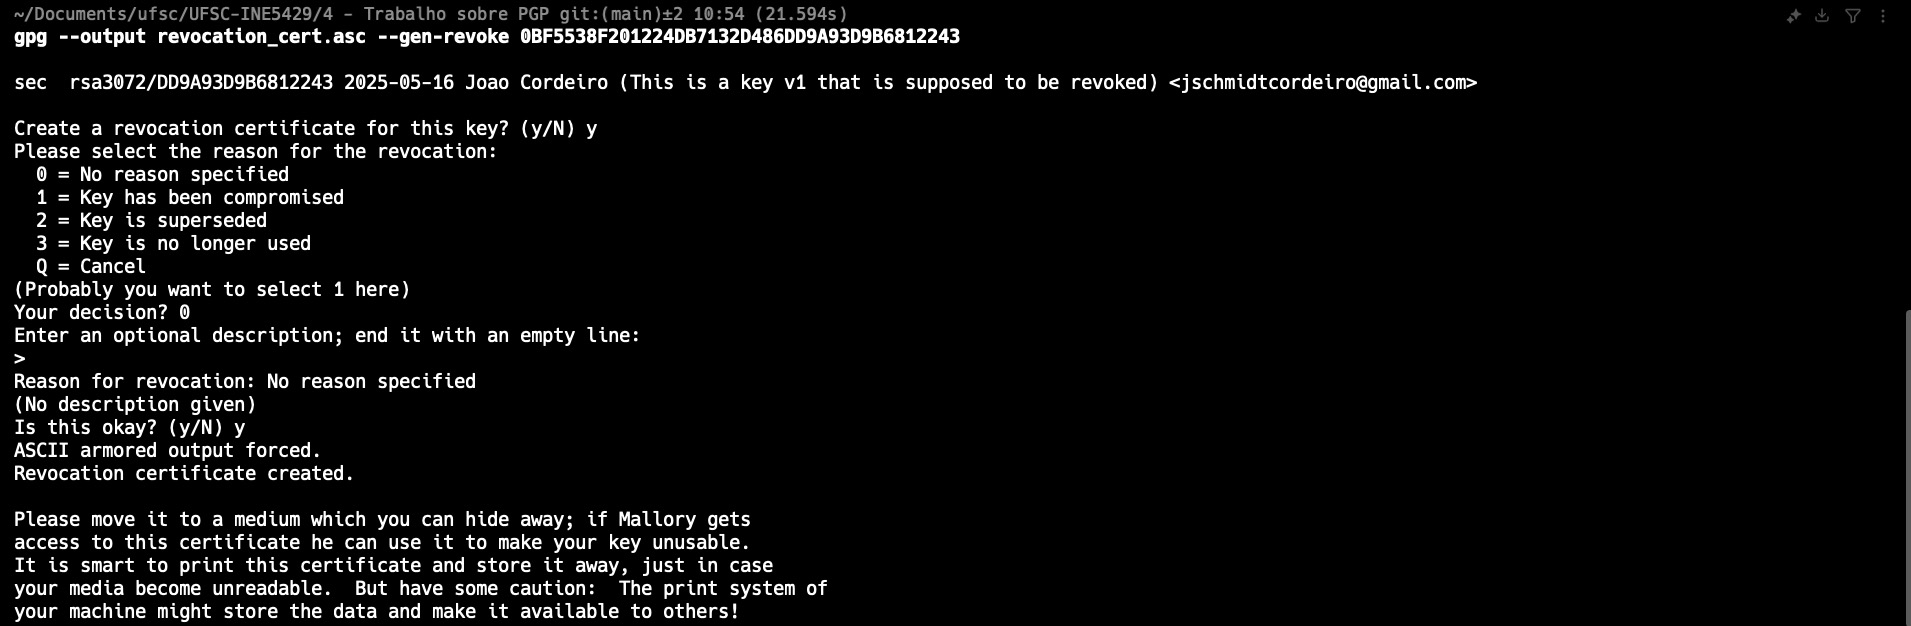
\includegraphics[width=0.8\textwidth]{images/02-criacao_certificado_revogacao.jpg}
    \caption{Criação do certificado de revogação}
    \label{fig:criacao-cert-revogacao}
\end{figure}

Durante o processo interativo:
\begin{enumerate}
    \item Confirmei a criação do certificado de revogação
    \item Selecionei o motivo da revogação (0 = Sem motivo específico)
    \item Adicionei uma descrição (nesse caso, foi adicionada uma descrição vazia)
    \item Confirmei a criação do certificado
\end{enumerate}

\section{Revogação do Certificado}
Com o certificado de revogação gerado, procedi à revogação da chave \cite{rfc4880}:

\begin{lstlisting}[language=bash]
# Importo o certificado de revogação para o chaveiro local
gpg --import revocation_cert.asc

# Envio a chave revogada para o servidor
gpg --keyserver keyserver.ubuntu.com --send-key 0BF5538F201224DB7132D486DD9A93D9B6812243
\end{lstlisting}

\begin{figure}[!htb]
    \centering
    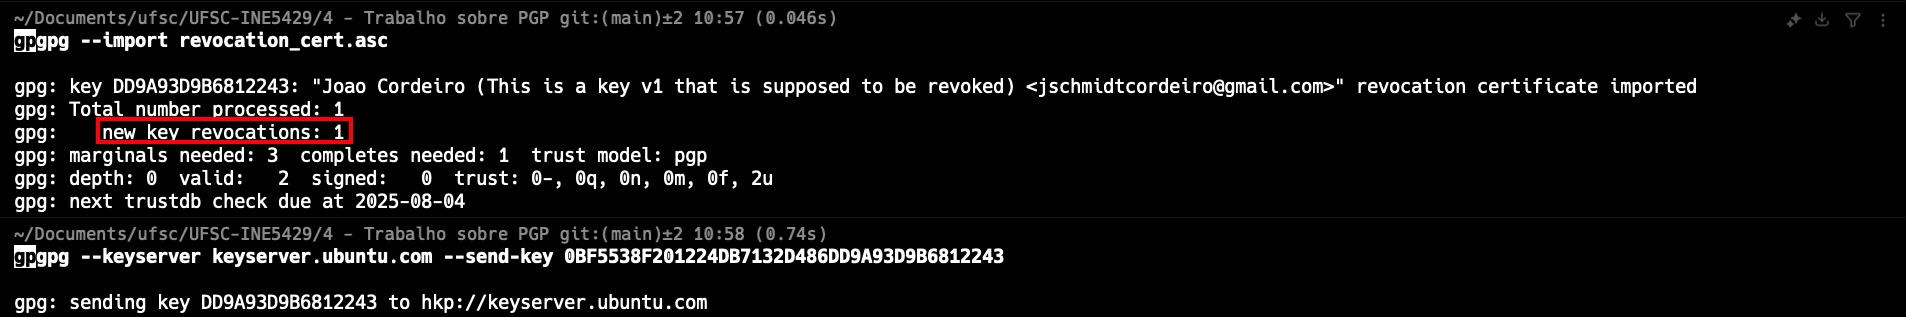
\includegraphics[width=0.8\textwidth]{images/02-revogacao_chave.jpeg}
    \caption{Revogação da chave}
    \label{fig:revogacao-chave}
\end{figure}

\section{Verificação da Revogação}
Para confirmar que a chave foi revogada com sucesso:

\begin{lstlisting}[language=bash]
# Atualizo o chaveiro local
gpg --keyserver keyserver.ubuntu.com --refresh-keys

# Verifico o status da chave
gpg --list-keys jschmidtcordeiro@gmail.com
\end{lstlisting}

\begin{figure}[!htb]
    \centering
    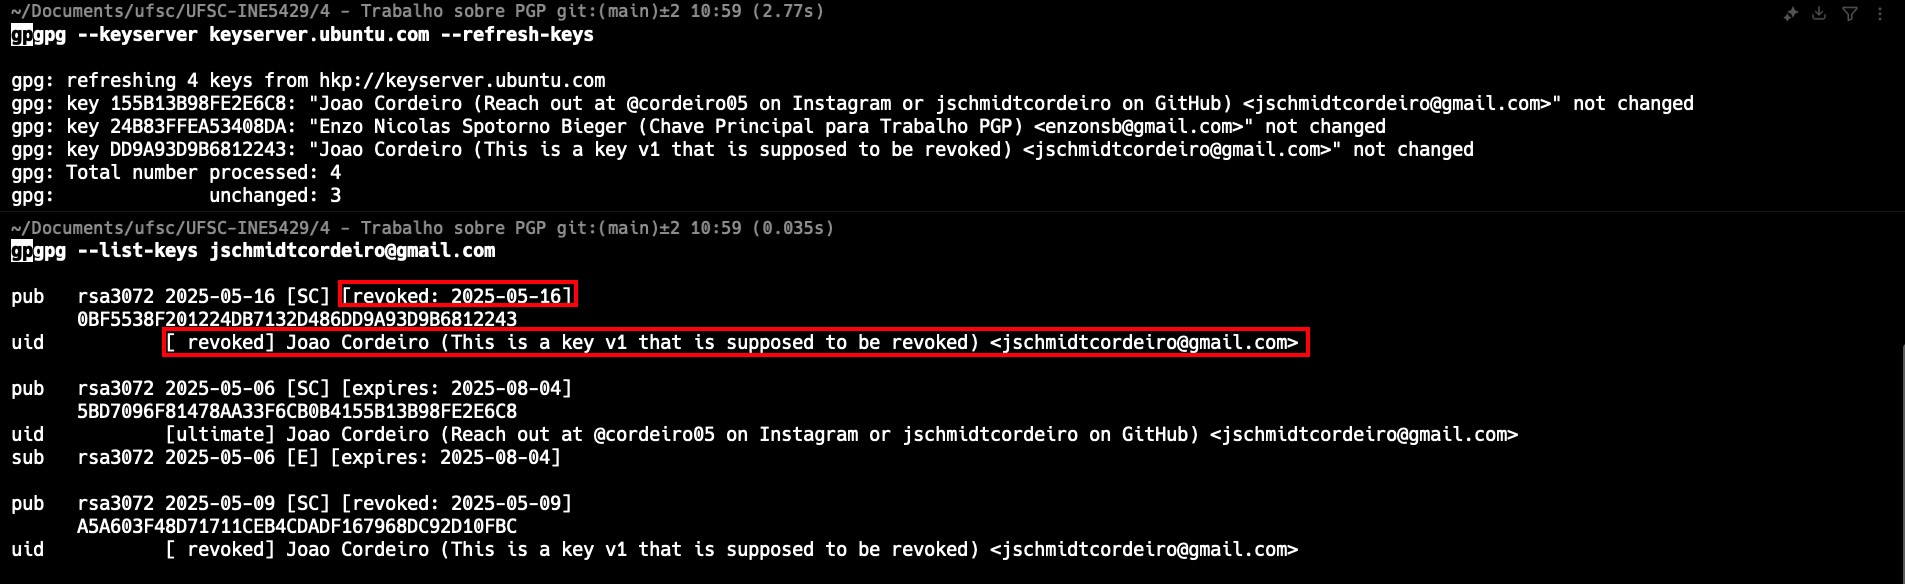
\includegraphics[width=0.8\textwidth]{images/02-verificacao_revogacao_chave.jpeg}
    \caption{Verificação da revogação}
    \label{fig:verificacao-revogacao}
\end{figure}

A saída indicou que a chave foi revogada, geralmente com uma marcação como "rev" ou "revoked".

\section{Resultados do Experimento}

Os resultados de cada comando dos experimentos estão disponíveis nas capturas de tela em suas respectivas seções, visando a facilidade de visualização e comparação. Abaixo se encontram as informações principais sobre o certificado revogado.

\begin{itemize}
    \item \textbf{KeyID do certificado revogado}: 0BF5538F201224DB7132D486DD9A93D9B6812243
    \item \textbf{Data da criação}: 16 de maio de 2025
    \item \textbf{Data da revogação}: 16 de maio de 2025
\end{itemize} 